% ==================================================
% CHAPTER 5: Using cosmic muons to measure relative strip position offsets %
% ==================================================

\chapter{Using cosmic muons to measure relative strip position offsets}
\label{chap:cosmics}
% Edit count: Lia - 0, Brigitte - 0

At McGill University, among other quality and functionality tests, each Canadian-made quadruplet was characterized with cosmic muons. In this chapter, the experimental setup and how the data was analyzed to provide relative strip position offsets is presented. The analysis method was motivated by the how the measurements could be compared to measurements done with the x-ray method (chapter~\ref{chap:xray}) but also it stands alone as a characterization of the alignment between strips of different layers. The chapter begins with a brief introduction to cosmic rays.

% --------------------------------------------------
\section{Cosmic rays}
% --------------------------------------------------

The earth is being constantly bombarded by particles from the sun, galactic sources and extra galactic sources~-- collectively called cosmic rays~\cite{boezio_chemical_2012, zyla_review_2020}. Cosmic rays consist mostly of protons, but also heavier ions, gamma rays and the term sometimes includes neutrinos. The primary (initial) cosmic ray interacting with the atmosphere causes electromagnetic and hadronic showers of secondary particles. Hadronic showers result from the primary cosmic ray interacting strongly with the target of the atmosphere, resulting in an abundant production of pions. Charged pions predominantly decay to muons (there is a lesser contribution to the muon flux from kaons as well)~\cite{grieder_cosmic_2001}. The secondary muons are relativistic and thanks to time dilation their lifetime is extended as measured in the reference frame of earth, so a flux of approximately 1 muon\SI{}{\per\cm\squared\per\min} reaches the ground~\cite{zyla_review_2020}. Measuring the muon flux and energy spectrum reveals information about primary cosmic rays~\cite{grieder_cosmic_2001} which is interesting to high energy physicists and astrophysicists. The muon flux is also terribly convenient for testing muon detectors.

% --------------------------------------------------
\section{Experimental setup}
% --------------------------------------------------

\begin{figure}[h]
    \centering
    \includegraphics[width = 0.9\textwidth]{figures/figure_test_bench.png}
    \caption{Cosmic muon hodoscope at McGill University with a sTGC quadruplet module in the test bench.}
    \label{fig:hodoscope}
\end{figure}

Cosmic muon characterization of sTGC quadruplet modules was done with a hodoscope, a complete description of which can be found in~\cite{lefebvre_thesis}. The quadruplet was placed in the center of the test bench. Above and below it was a layer of scintillator-PMT arrays, as shown in figure~\ref{fig:hodoscope}. When a cosmic muon passed within the acceptance of the hodoscope, at least one scintillator from the top array and at least one from the bottom array fired in coincidence. A trigger signal was formed using NIM modules from the coincidence of signals from the top and bottom arrays of scintillators. The trigger signal was passed \iffalse through a KC705\footnote{Xilinx, Xilinx Kintex-7 FPGA KC705 Evaluation Kit, EK-K7-KC705-G, 2018} which sent it \fi to the front-end electronics attached to the adaptor boards of each layer of the quadruplet.

Operating the chambers also required gas and high voltage. A gas mixture of pentane-CO$_{2}$ in the appropriate proportions was prepared and delivered to each sTGC with a gas system designed and made at McGill University~\cite{keyes_development_2017}. Since pentane is flammable, the gas system was designed with safety top of mind. The gas system was controlled by a slow control program, also custom made~\cite{keyes_development_2017}. To prepare the quadruplets for operation, CO$_{2}$ was flushed through them overnight to remove potential impurities within each chamber's gas volume. Then, the equivalent of approximately five sTGC gas volumes of the pentane-CO$_{2}$ mixture was flushed through to ensure a uniform gas mixture inside the sTGCs; the procedure takes approximately four hours. High voltage was provided by commercial CAEN high voltage boards~\cite{keyes_development_2017}. 

% About 2.9 kV vs 3.1 kV
%Although the chambers will be operated at 2.8~kV in ATLAS, the earlier version of the FEBs used at McGill had a worse signal-to-noise ratio for pads, which was compensated for operating the chambers at 3.1~kV, which increased the chambers' gain. Operating at 2.9~kV was sufficient for strip and wire signals and closer to the nominal voltage. Collecting 1 million triggers at each voltage provided enough statistics to calculate characterization metrics, which meant collecting data for just over two hours per quadruplet per voltage.

% --------------------------------------------------
\section{Data acquisition}
% --------------------------------------------------
% It would be great to have a scope trace here, preferably of a strip. Oops.
Each sTGC electrode was connected to a channel on a prototype ASIC\footnote{A custom Application Specific Integrated Circuit (ASIC) named VMM3~\cite{iakovidis_vmm3_2017}, designed for the readout of signals from the micromegas and sTGCs of the NSWs.} on the front-end electronics, attached to the adaptor boards on each layer of a quadruplet. Each ASIC features 64 charge amplifiers with selectable gain and input signal polarities, which output the digitized amplitude of the signal at peak for channels above a pre-defined threshold. Thresholds were estimated~\cite{chen_calibration_2019} by optimizing the efficiency of detecting muons while minimizing noise, and further manually tuned in the configuration/readout software before the start of data acquisition for each quadruplet. The signal from the capacitively-coupled strip electrodes has positive polarity and is read out with a gain of one. For each trigger, the signal peak amplitude of all channels above threshold was recorded  as an event and stored in a binary file. The readout of strips made use of a special feature of the custom ASIC, the so-called ``neighbour triggering'' function where signals on channels adjacent to those above threshold are also read out.

The quadruplets were held at 3.1~kV for approximately two hours to collect data from approximately 1~million muon triggers.

% --------------------------------------------------
\section{Data preparation}
% --------------------------------------------------
\subsection{Data quality cuts on electrode hits}
\label{subsec:hit_cuts}
Corrupted data, if any, is removed while the raw data is being recorded in a binary file. After data taking is completed, the raw data is decoded and the electronics channels are mapped to physical readout electrodes of the quadruplet. The result of this data preparation step is stored in a \package{ROOT}~\cite{ROOT_paper} tree data format. 

A hit is defined as a signal recorded from a channel that was above threshold or (in the case of strips) neighbour triggered. In addition to hits from muons, the quadruplets record noise from the electronics and $\delta$-rays (electrons liberated with sufficient energy to escape a significant distance away from the primary radiation and produce further ionization). Therefore, selection cuts are applied to reduce the number of hits that do not originate from muons. Readout strips located at the very edge of the cathode board tend to have higher electronic noise.  As a result, all strip hits on a layer where a hit is present on the strips at either edge of the quadruplet are removed from the analysis. A default pedestal value is subtracted from the recorded signal peak amplitude of each electrode for a more realistic estimate of the signal amplitude. Also, events that only have hits on pad electrodes (no strips or wires) were removed from the analysis since these hits are likely from electronic noise, which is higher on the pad readout channels due to their large area.

% --------------------------------------------------
\subsection{Clustering and tracking}
% --------------------------------------------------
\label{subsec:clustering}
For events passing the quality selection cuts defined in section~\ref{subsec:hit_cuts}, the $x$- and $y$-coordinates of the ionization avalanche on each layer are extracted from the signal on the wires and strips respectively for each event, as shown schematically in figure~\ref{fig:mwpc_coords}. In this work, $x$ is defined as the coordinate perpendicular to the wires and $y$ is defined as the coordinate perpendicular to the strips. The $z$-coordinate is perpendicular to the sTGC surface.

The $x$-coordinate of the muon position is taken as the center of the wire group with the maximum peak signal amplitude, since the wire groups' pitch (\SI{36}{\milli\meter}) is larger than the typical extent of the ionization charge generated inside a sTGC. Assuming that the true $x$-position of the hit is sampled from a uniform distribution over the width of the wire group, the uncertainty in the x-position is approximately $\frac{36}{\sqrt{12}}$~mm~=~10~mm~\cite{Sauli:117989}.

\newpage
\thispagestyle{empty}
\newgeometry{top=0.5in,bottom=0.5in}
\begin{figure}
    \centering
    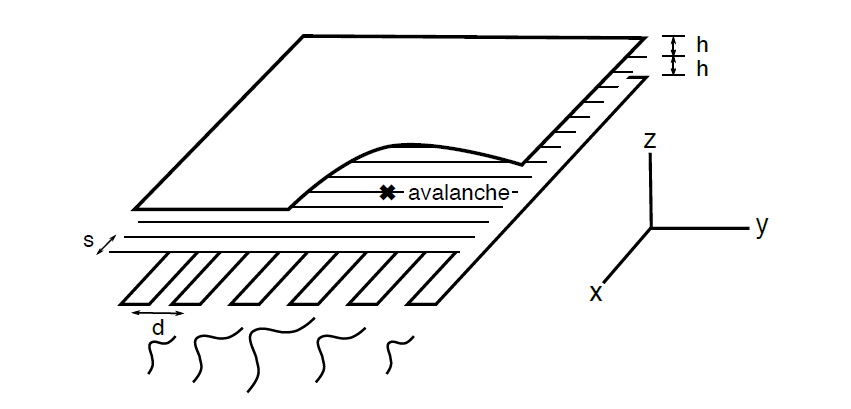
\includegraphics[width = 0.8\textwidth]{figures/mwpc_lefebvre_thesis_gatti.png}
    \caption{Schematic diagram representing the three types of electrodes in a sTGC detector. The position of the ionization avalanche is extracted from the wires and strips that picked up the avalanche signal. The signals on individual strips are sketched. Clustering is the process by which a Gaussian function (represented by the grey dashed line) is fitted to the distribution of the signal amplitude on individual contiguous strips; a sample cluster is shown in figure~\ref{fig:sample_cluster}. In this work, the $x$($y$)-coordinate will always refer to the coordinate perpendicular to the wires (strips). The $z$-coordinate is perpendicular to the sTGC surface~\cite{lefebvre_thesis, gatti_optimum_1979}.}
    \label{fig:mwpc_coords}
%\end{figure}
    \vspace*{\floatsep}
%\begin{figure}
    \centering
    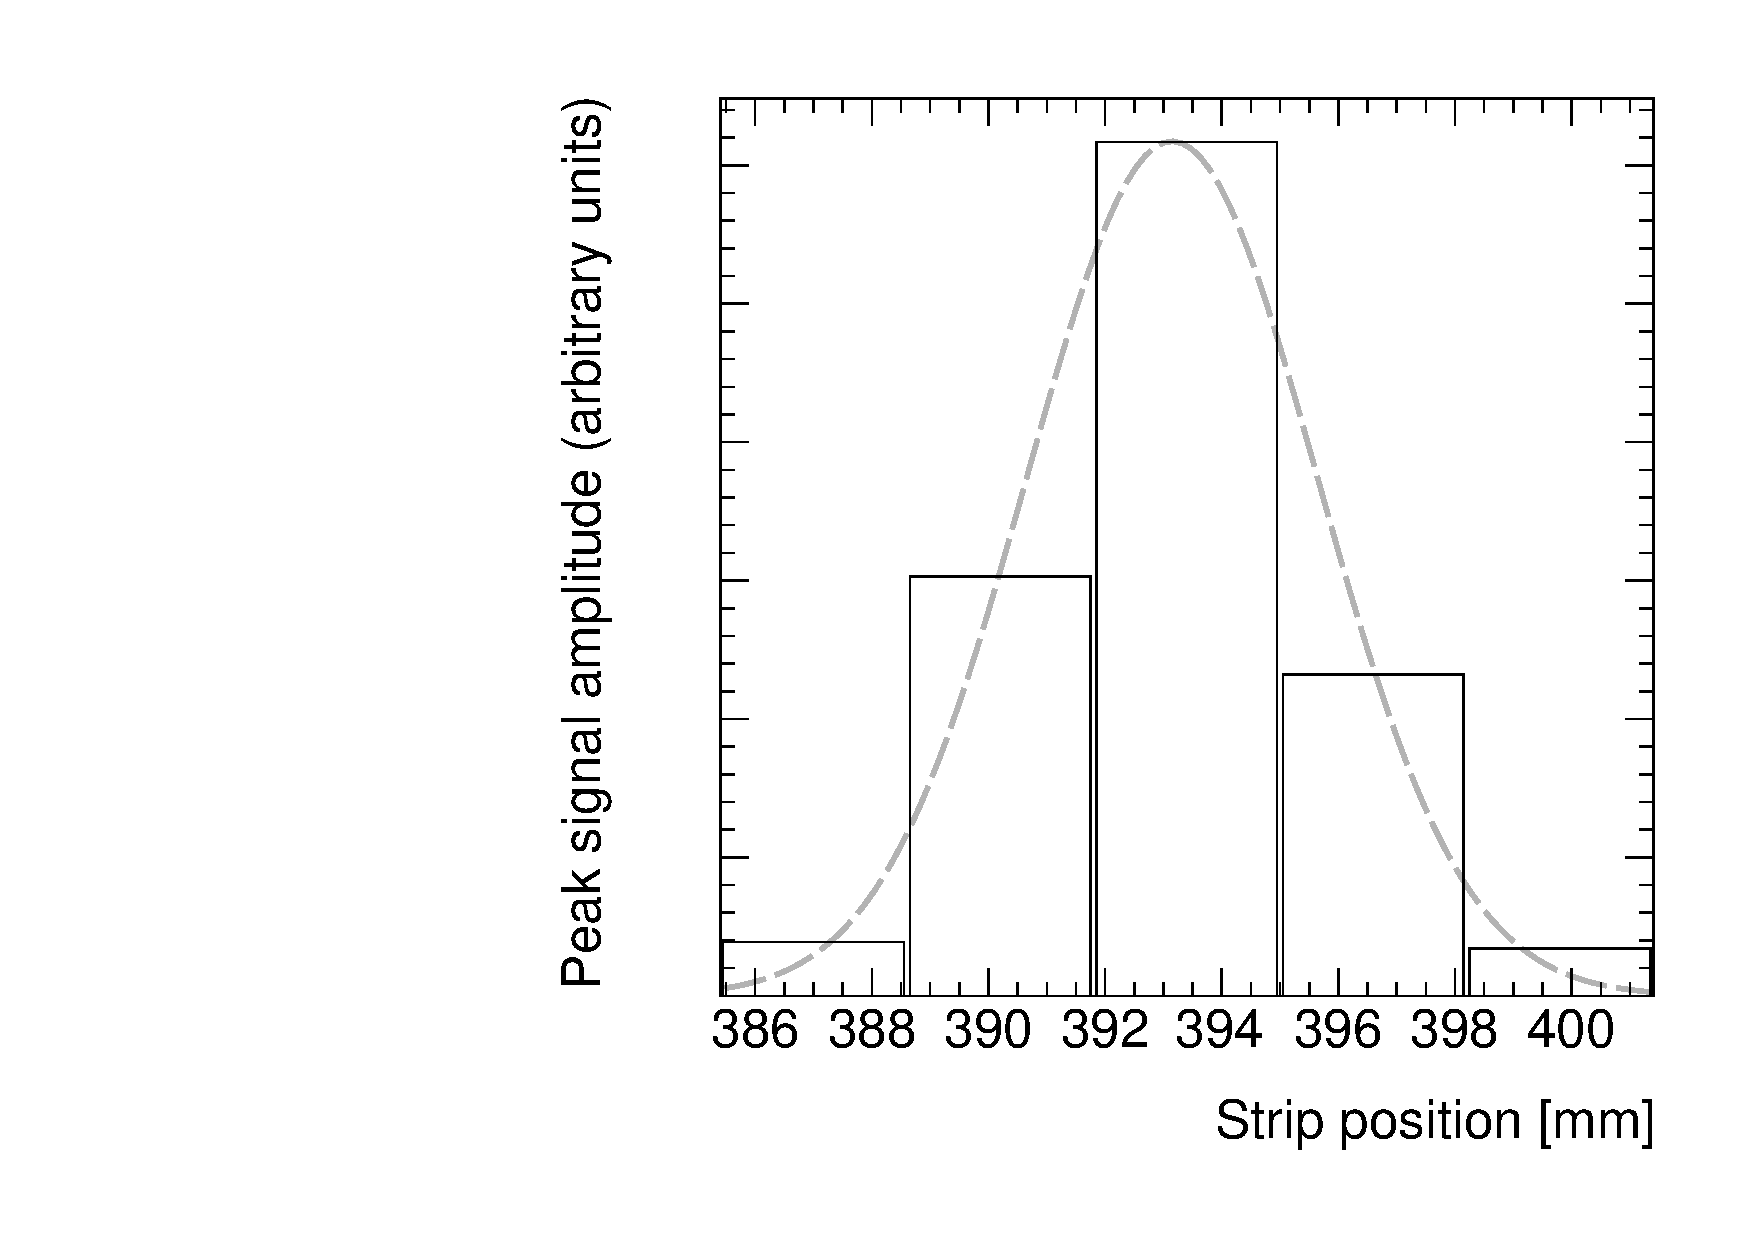
\includegraphics[width = 0.5\textwidth]{figures/sample_cluster_QL2C04_event5_layer2.pdf}
    \caption{A sample cluster resulting from signal recorded on a group of contiguous strips after the passing of a muon. The grey dashed line represents the result of a fit to a Gaussian distribution.}
    \label{fig:sample_cluster}
\end{figure}
\newpage
\restoregeometry

The $y$-coordinate of the muon's position is taken as the Gaussian mean of the peak signal amplitude distribution across a group of contiguous strips that registered hits. The process of grouping contiguous strip hits on a layer is called clustering, and the resulting group is called a cluster. Figure~\ref{fig:mwpc_coords} sketches the clustering process and a sample cluster is shown in figure~\ref{fig:sample_cluster}. The data acquisition system recorded the identification number of the strip electrode that was hit and in the clustering process the position of the center of the strip electrode is calculated based on the nominal quadruplet geometry. Typically, clusters are built of 3-5 strips. The thickness of the graphite coating over the cathode boards determined how many strips picked up the ionization image charge. Larger clusters can often originate from $\delta$-rays since they spread the ionization charge over a larger area.

Events are removed from further analysis if there are two reconstructed clusters on one sTGC, since some hits could be from electronic noise or a simultaneous second muon traversing the chamber. Clusters are rejected if the cluster size is lesser than three strips (which should not happen for real events thanks to neighbour triggering), and if the cluster size is greater than 25. After all quality selection cuts are applied on hits and clusters, approximately half of the events recorded remain.

The uncertainty on the reconstructed cluster position is assessed by comparing the difference between Gaussian means obtained using two different algorithms. As shown in appendix~\ref{appendix:clustering}, the difference between the means from the two algorithms considered is found to be approximately \SI{60}{\micro\meter} on average, larger than the statistical uncertainty on the Gaussian mean obtained from the cluster fit. Therefore, an uncertainty of \SI{60}{\micro\meter} is assigned to the reconstructed y-coordinate of a muon. 

The reconstructed $x$ and $y$ coordinates on each quadruplet layer are used to reconstruct a straight track, independently, in the $x$-$z$ and $y$-$z$ planes. Tracks are reconstructed using muon coordinates for every possible pair of two sTGC layers.  For example, if an event has muon coordinates reconstructed on all four layers, a total of six track segments in the $x$-$z$ plane and six track segments in the $y$-$z$ plane will be reconstructed. 

%TODO : Include hit and track map? - yes if Brigitte says you need a num_entries plot in chapter 3. You didn't include it because you never mention wire supports in TH2 analysis. But if you want to add num entries for clarity, include cluster map here. Cluster map > raw hits because less cuts and gets across the idea that x is just hit or no hit while y comes from clustering.  

% Edit count: Lia - 2, Brigitte - 0

% --------------------------------------------------
\section{Relative local offsets}
% --------------------------------------------------

The offset of a strip from its nominal position can be modeled as a passive transformation. The \textit{local offset} is defined as the shift in the strip pattern with respect to nominal geometry in a specific area of the sTGC. Local offsets systematically change the set of strips nearest to muons passing through an area. The data preparation software assumes that strips are in their nominal positions, so the recorded $y$-coordinate of the muon on layer $i$, $y_i$, is shifted opposite to the layer's local offset, $d_{local, i}$, by
% Maybe useful sentence?: The local offset is a result of the non-conformities in the strip pattern etching and inter-layer misalignments.
\begin{equation}
    y_i = y_{nom, i} - d_{local, i},
    \label{eqn:local_translation}
\end{equation}
% Maybe useful sentence?: The true position of individual cosmic muons is not known, and in the analysis the four detector planes float with respect to a software-implemented origin that is not associated with a fixed physical location.
where $y_{nom, i}$ is the position of the muon that would have been recorded on layer $i$ if there was no local offset. Equation~\ref{eqn:local_translation} ignores other factors that affect the cluster position, like position resolution. With cosmics data, there was no external reference to measure $y_{nom, i}$ and the local offset is unknown. Therefore, only relative local offsets can be measured. 

% Potential BREAK for Motivation section at beginning ^
To measure relative local offsets, two of the four sTGC layers are chosen to provide a reference coordinate system. Relative local offsets are calculated with respect to the two reference or fixed layers. The hits on the two fixed layers were used to create tracks that can be interpolated or extrapolated (polated) to the other two layers. The set of two fixed layers and the layer polated to are referred to as a tracking combination. The residual of track $i$, $\Delta_i$, is defined as,
\begin{equation}
    \Delta_i = y_{i} - y_{track, i},
    \label{eqn:residual}
\end{equation}

where $y_{track, i}$ is the polated track position on the sTGC layer the residual is measured on. Track residuals are affected by the local offset in the area of each layer's hit. As an example, in figure~\ref{fig:fake_event_display}, the residual on layer 2 perhaps indicates that layer 2 is offset with respect to layers 1 and 4 in the area of the track. Of course, a single track residual says nothing of the real relative local offset because of the limited spatial resolution of the detectors and fake tracks caused by noise or delta rays. However, the mean of residuals for all tracks in a region of interest will be shifted systematically by the local offsets between layers~\cite{lefebvre_thesis}. For a quadruplet with nominal geometry, the mean of residuals should be zero in all regions and for all reference frames, unlike the example regions in figure~\ref{fig:res_dist}. The value of the mean of residuals is a measure of the relative local offset of the layer with respect to the two fixed layers used to reconstruct the muon track. The sign convention is such that the mean of residuals is opposite to the relative local offset.

\begin{figure}
    \centering
    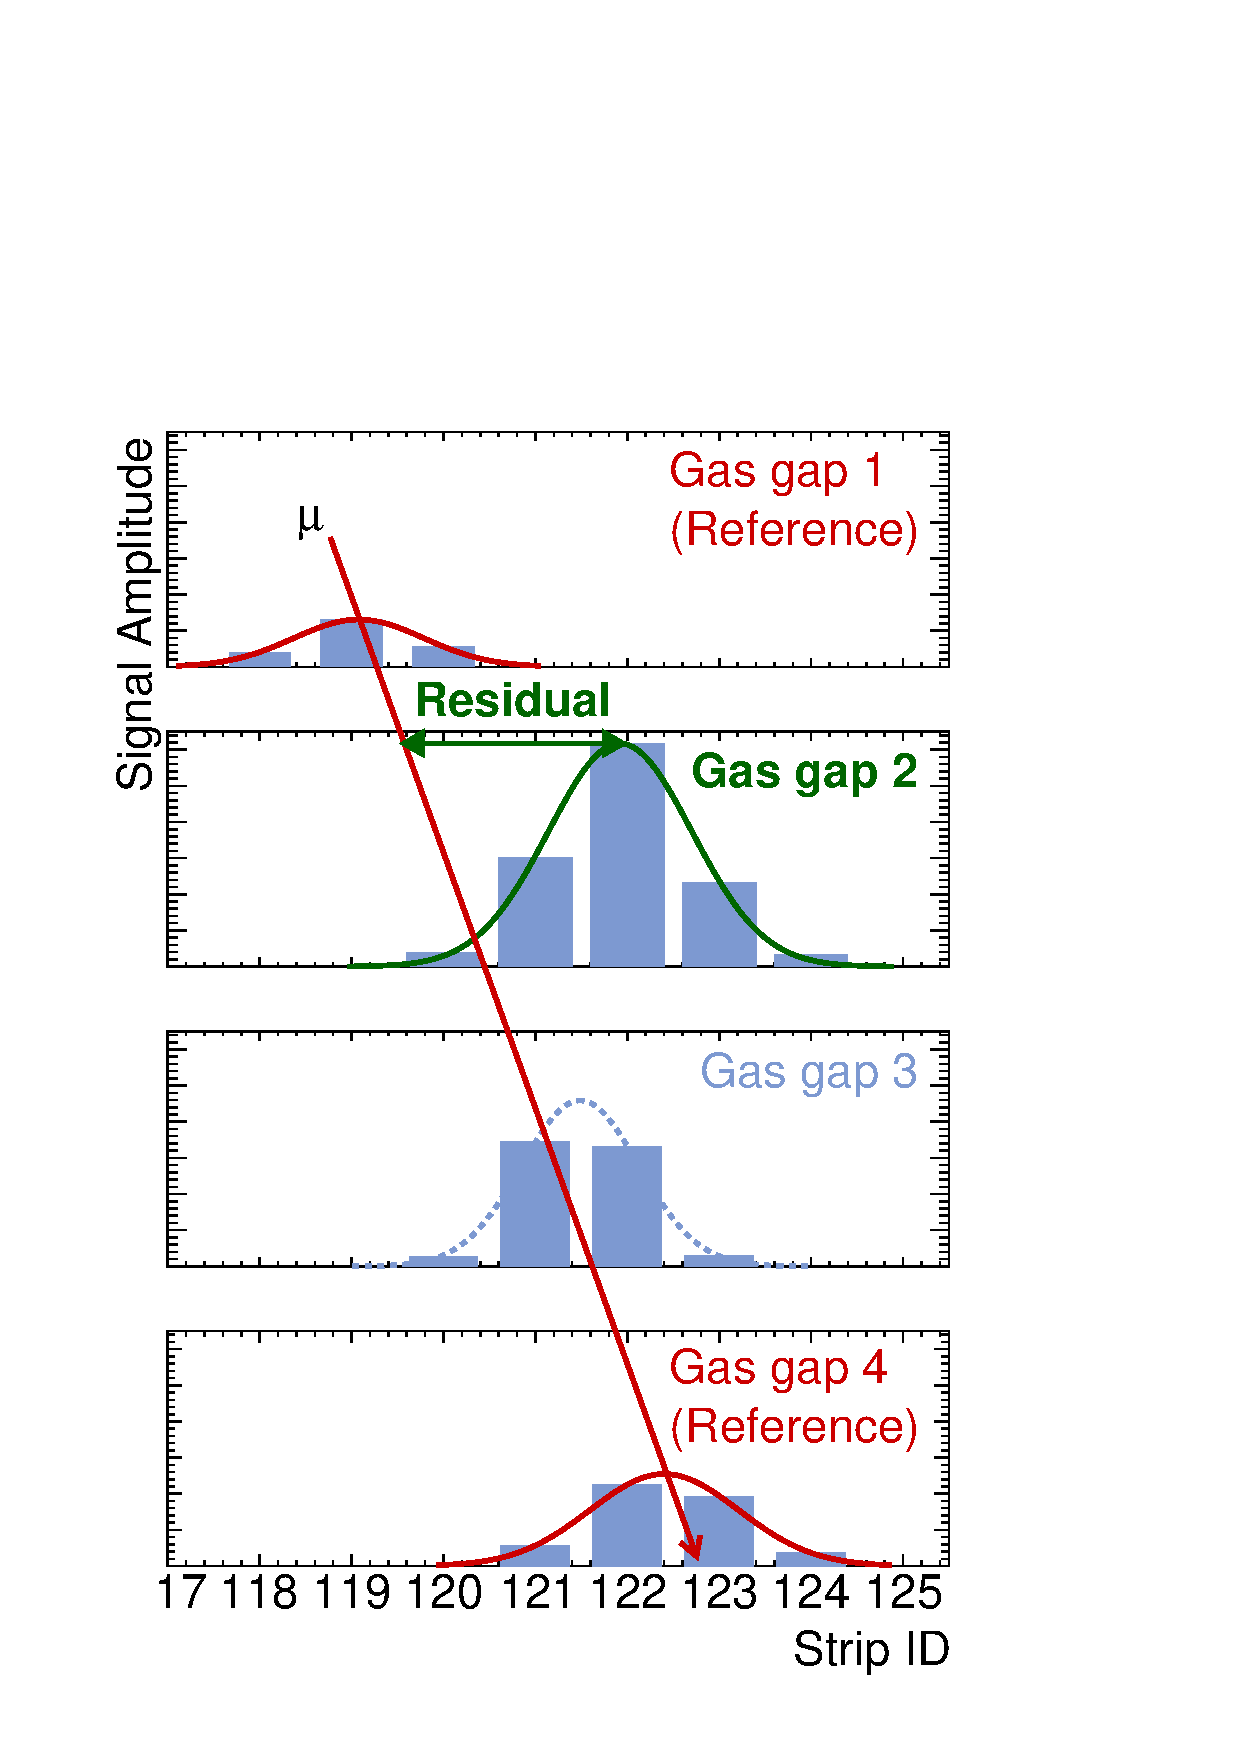
\includegraphics[width = \textwidth]{figures/figure_fake_event_display.pdf}
    \caption{Representation of a muon event recorded by an sTGC quadruplet. The charge clusters measured using strip electrodes are fit with a Gaussian distribution and the fitted mean is taken as the reconstructed muon position. A track is built from the chosen reference layers, 1 and 4, and the track residual is calculated on layer 2. The clusters come from a real muon, but their positions were modified to highlight the non-zero value of the residual on layer 2.}
    \label{fig:fake_event_display}
\end{figure}

\begin{figure}
\centering
\begin{subfigure}{.5\textwidth}
  \centering
  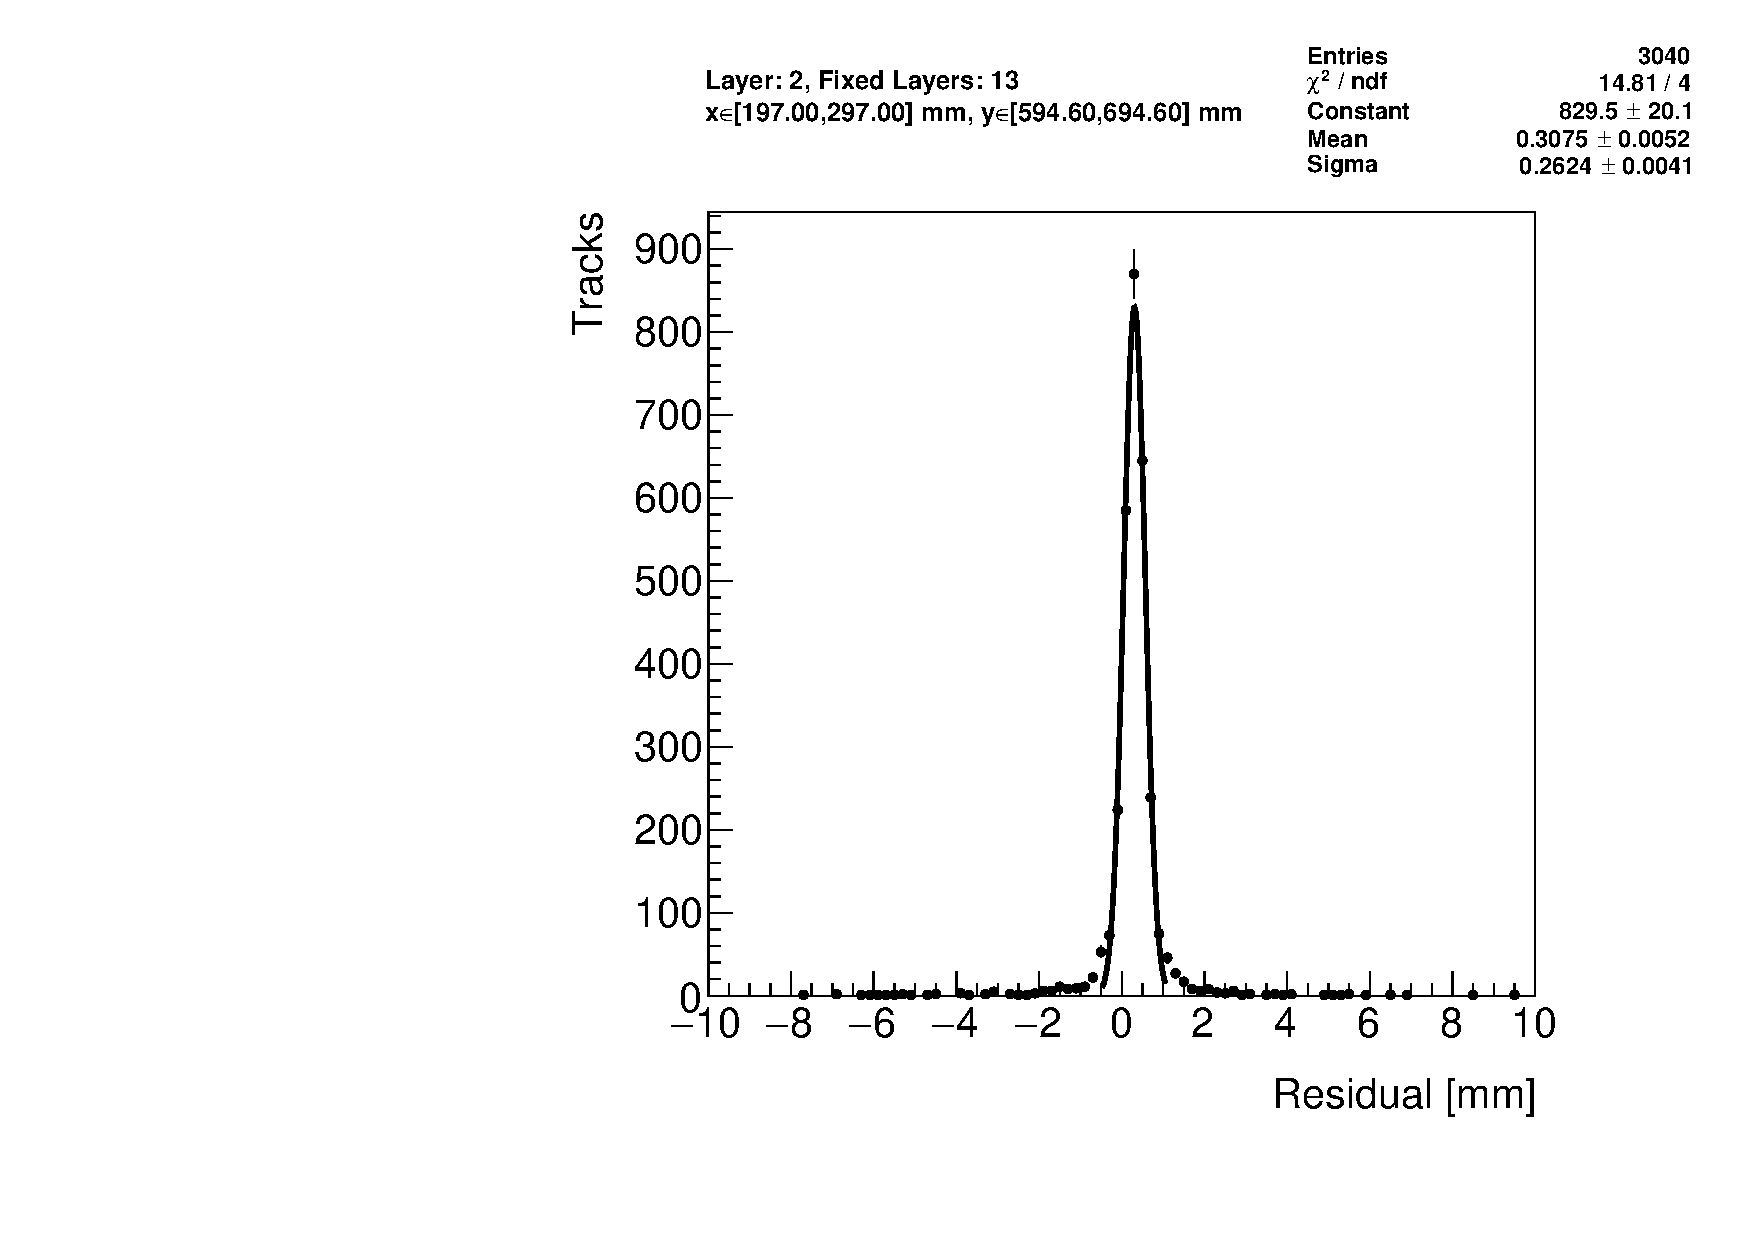
\includegraphics[width=\linewidth]{figures/figure_res_dist_QL2P11_3100V_2021-08-05_xbin_12_ybin_7_layer2_fixedlayers13.pdf}
  \caption{Tracks on layer 2, reference layers 1 and 3.}
  \label{fig:res_dist_L2_F13}
\end{subfigure}
\begin{subfigure}{.5\textwidth}
  \centering
  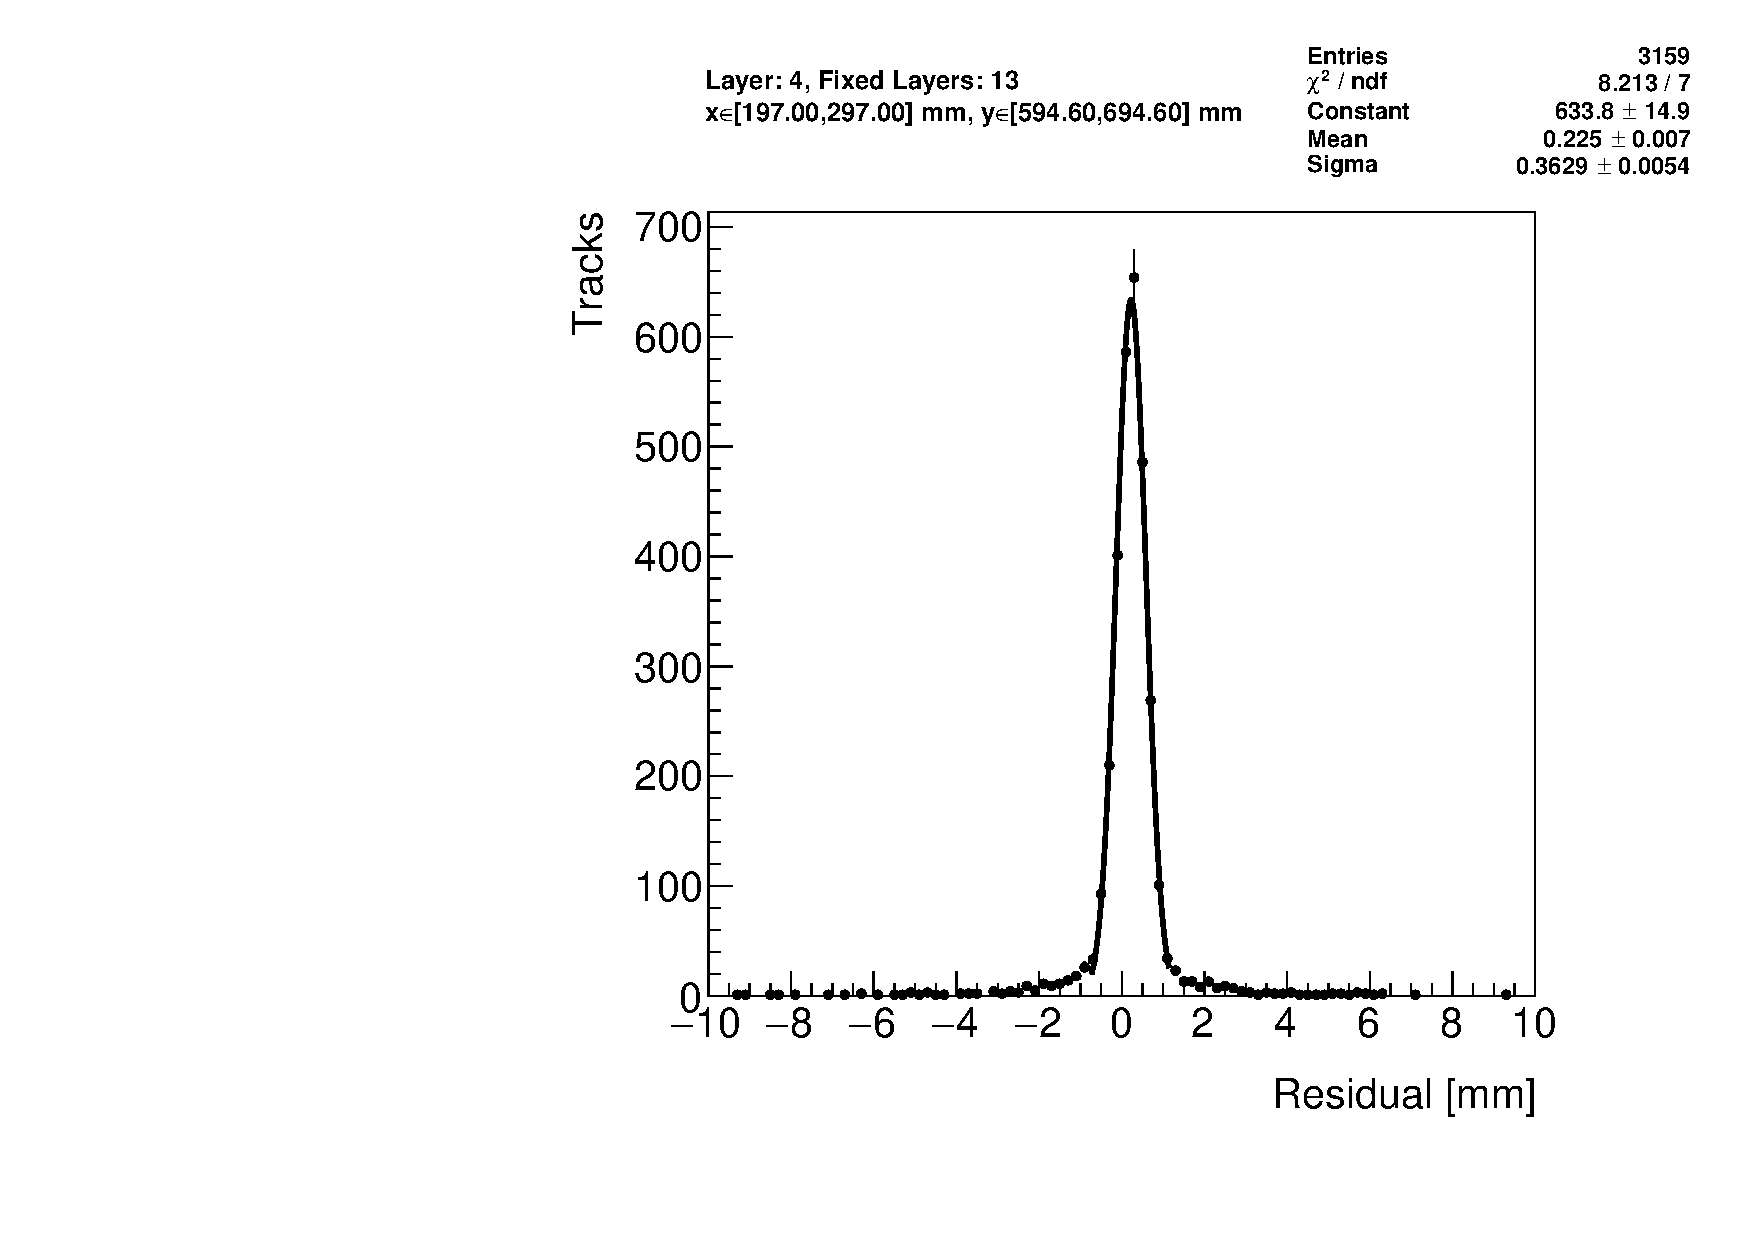
\includegraphics[width=\linewidth]{figures/figure_res_dist_QL2P11_3100V_2021-08-05_xbin_12_ybin_7_layer4_fixedlayers13.pdf}
  \caption{Tracks on layer 4, reference layers 1 and 3.}
  \label{fig:res_dist_L4_F13}
\end{subfigure}
\caption{Residual distribution in the region $x\in\left[197, 297\right]$~mm,  $y\in\left[594.6, 694.6\right]$~mm (\SI{100}{mm} by \SI{100}{mm} area) for two different tracking combinations. Data from quadruplet QL2.P.11.}
\label{fig:res_dist}
\end{figure}

To study the relative local offsets, residual distributions across each strip layer of a quadruplet for all possible tracking combinations are assembled and fitted. As expected, the residual distributions are wider for tracking combinations where the extrapolation lever arm is largest, as in the example distributions shown in figure~\ref{fig:res_dist}. In general, residual means from distributions of residuals with geometrically less favourable tracking combinations have larger statistical and systematic uncertainties. The bin size of \SI{200}{\micro\meter} for the distributions shown in figure~\ref{fig:res_dist} was chosen based on the uncertainty on residuals calculated from tracks on layer 4 (1) built from hits on layers 1 and 2 (3 and 4) given a cluster $y$-coordinate uncertainty of \SI{60}{\micro\meter} (discussed in section~\ref{subsec:clustering} and appendix~\ref{appendix:clustering}), since these tracks yield residuals with the largest uncertainties.

A Gaussian fit is used to extract the mean of the residual distributions. The residual distributions are actually better modeled by a double Gaussian distribution, which better captures the distribution tails in figure~\ref{fig:res_dist}. However, a study described in appendix~\ref{appendix:systematics_res_fit_fcn} found that a fit to a single Gaussian function in the core of the distribution is sufficient to reconstruct the mean of the distribution.

The area of the region of interest where tracks residuals were included in the residual distribution was \SI{100}{\milli\meter} by \SI{100}{\milli\meter}. The size balanced the number of tracks falling in the region of interest to give a small statistical uncertainty on the fitted mean while being smaller than the order on which local offsets were expected to change significantly. ``Significantly'' was defined as \SI{100}{\micro\meter}, the required position resolution of the sTGCs and the precision to which strip positions should be known. The distance over which local offsets are expected to change significantly can be estimated using a simple alignment model. Assuming the strips of a layer have been displaced uniformly from their nominal positions by a global offset and rotation, the distance in $x$ that a large but possible rotation of \SI{1}{mrad} changes the local offset by \SI{100}{\micro\meter} is \SI{100}{mm}.

% Original position of this paragraph
% It is only possible to calculate relative local offsets with cosmics data because there was no external reference to measure positions on all layers with respect to. As an example, assuming that the residual on layer 2 in figure~\ref{fig:fake_event_display} is representative of the relative local offset, the residual on layer 2 could be caused by the strips on layer 2 being misaligned from nominal, but it could also be caused by strips on layers 1 and 4 being misaligned from nominal while the strips on layer 2 are in their nominal positions! Any number of combinations of local offsets on layers 1, 2 and 4 could produce the residual on layer 2. The value of relative local offset measurements will be shown and discussed throughout this work.
The means of residuals are plotted across each sTGC layer for every possible tracking combination to get a picture of the how the relative local offsets change as a function of position over the layer's surface. Figure~\ref{fig:res_mean_th2} shows the mean of residuals on layer 2 calculated with layers 1 and 3 as reference for two different quadruplets, referred to as QL2.P.11 and QL2.P.8. In figure~\ref{fig:res_mean_th2_ql2p11}, the Gaussian mean of the residual distribution in figure~\ref{fig:res_dist_L2_F13} is the entry in the bin defined by the  boundaries $x\in\left[197, 297\right]$~mm,  $y\in\left[594.6, 694.6\right]$~mm.

Many of the residual means are non-zero and change smoothly over layer 2, indicating that there are relative local offsets stemming from global misalignments between the strip patterns of different sTGC layers in both quadruplets. Given that the residual mean changes with $x$ in figure~\ref{fig:res_mean_th2_ql2p11}, quadruplet QL2.P.11 likely has a rotation of layer 2 with respect to layers 1 and 3, combined with an offset of the entire layer. The residual means are smaller in figure~\ref{fig:res_mean_th2_ql2p8} indicating that quadruplet QL2.P.8 is less misaligned overall than QL2.P.11; however, the relative local offsets range between $\pm$\SI{200}{\micro\meter} so they are significant enough to warrant a correction so the quadruplet can achieve the required track angular resolution in the NSW.

\newpage
\thispagestyle{empty}
\newgeometry{top=0.5in,bottom=0.5in}
\begin{figure}
\centering
\begin{subfigure}{\textwidth}
  \centering
  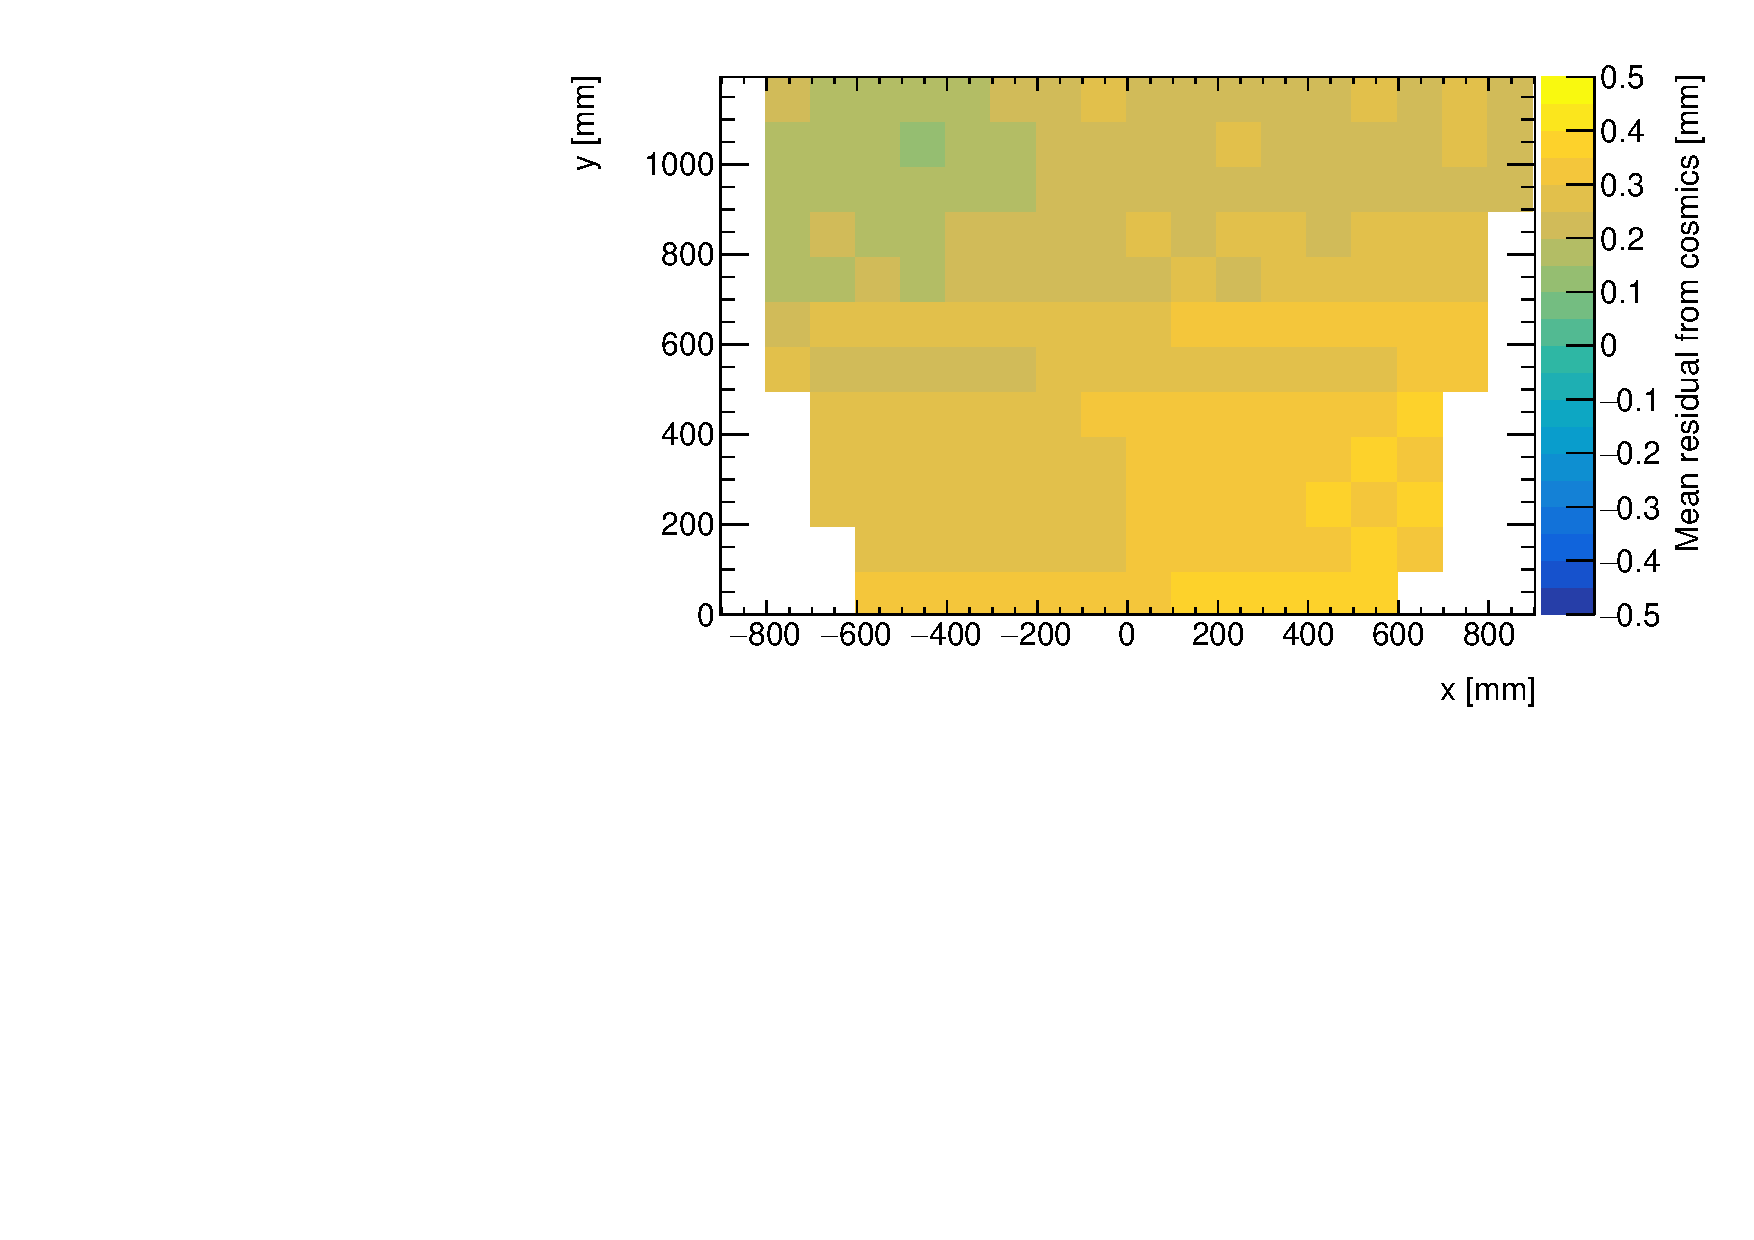
\includegraphics[width=\linewidth]{figures/figure_QL2P11_3100V_2021-08-05_th2_means_layer2_fixedlayers13.pdf}
  \caption{Mean of track residuals on layer 2, obtained using layers 1 and 3 as reference, for QL2.P.11.}
  \label{fig:res_mean_th2_ql2p11}
\end{subfigure}%
\vspace*{\floatsep}
\begin{subfigure}{\textwidth}
  \centering
  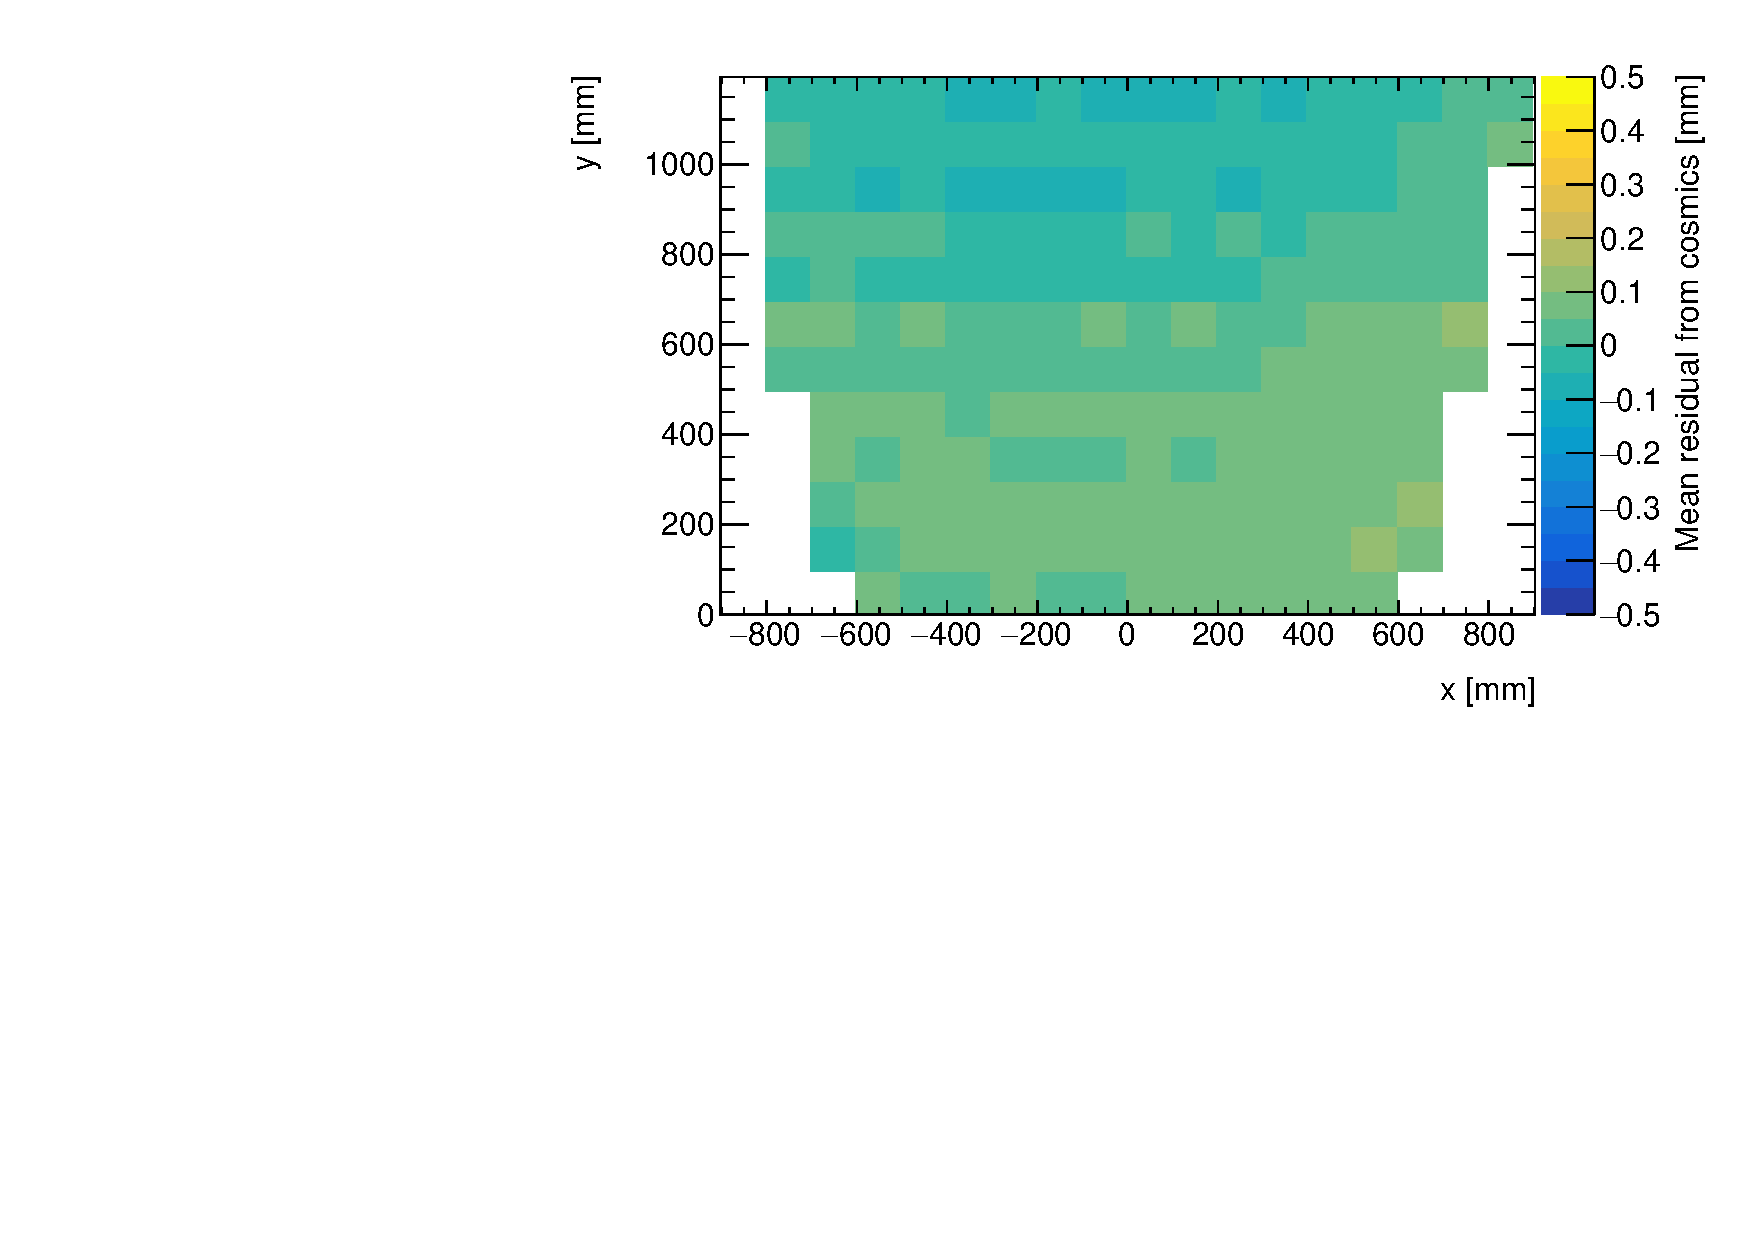
\includegraphics[width=\linewidth]{figures/figure_QL2P08_3100V_2021-08-03_th2_means_layer2_fixedlayers13.pdf}
  \caption{Mean of track residuals on layer 2, obtained using layers 1 and 3 as reference, for QL2.P.8.}
  \label{fig:res_mean_th2_ql2p8}
\end{subfigure}
\caption{Mean of residuals in each \SI{100}{\milli\meter} by \SI{100}{\milli\meter} bin over the area of sTGC layer 2 for quadruplets QL2.P.11 and QL2.P.8. The entry in $x\in\left[197, 297\right]$~mm,  $y\in\left[594.6, 694.6\right]$~mm of figure~\ref{fig:res_mean_th2_ql2p11} corresponds to the fitted Gaussian mean in figures~\ref{fig:res_dist_L2_F13}. The mean of residuals has the same value and opposite sign to the relative local offset of layer 2 with respect to the reference frame defined by layers 1 and 3.}
\label{fig:res_mean_th2}
\end{figure}
\newpage
\restoregeometry

% --------------------------------------------------
\section{Systematic uncertainty}
% --------------------------------------------------
\label{sec:cosmics_sys_uncerts}

The statistical uncertainty on the local residual means was typically around \SI{10}{} - \SI{20}{\micro\meter}, and appendix~\ref{appendix:statistics} shows that the analysis is not statistically limited by the number of triggers collected for each quadruplet. Systematic uncertainties were found to be larger than the statistical uncertainty on the residual means.

Several analysis choices had some degree of impact on the fitted means of local track residual distributions. To study the impacts, the residual means were calculated in different ways and distributions of the differences made. The complete studies are shown in appendix~\ref{appendix:systematics}. The root-mean-square (RMS) of the residual mean difference distributions were used to quantify the impact of the different analysis choices as systematic uncertainties on the residual means. The following analysis choices are considered:
\begin{itemize}
  \item The impact of performing a single or double Gaussian fit on the track residual distributions is studied. As shown in appendix~\ref{appendix:systematics_res_fit_fcn}, the difference between fitting the track residual distribution with a single or double Gaussian function varies between 10-\SI{30}{\micro\meter} from the most to least geometrically favourable tracking combinations.
  \item The impact of the operating voltage used during data taking is investigated. Cosmic muon data was recorded at 2.9~kV and 3.1~kV. As described in appendix~\ref{appendix:systematics_2900V_vs_3100V}, an uncertainty between 10-\SI{40}{\micro\meter} is assigned to the different tracking combinations.
  \item The impact of using different Gaussian fitting algorithms used to reconstruct the position of a charge cluster was considered. Clusters are fit with the Minuit2~\cite{hatlo_developments_2005} and Guo's method~\cite{guo_simple_2011}. As shown in appendix~\ref{appendix:systematics_cluster_fit_fcn}, the resulting difference in residual means is between 10-\SI{30}{\micro\meter} from the most to least geometrically favourable tracking combinations.
  \item The impact of correcting reconstructed cluster positions for differential non-linearity (DNL) is studied. DNL is fully described in appendix~\ref{appendix:systematics_dnl}. It is a bias in the reconstructed cluster position that comes from discretely sampling a continuous distribution, in this case the charge distribution~\cite{endo_systematic_1981, lefebvre_thesis, abusleme_performance_2016}. The difference between residual means is compared with and without correcting the reconstructed cluster positions. Appendix~\ref{appendix:systematics_dnl} shows that the impact of the correction is smaller than \SI{10}{\micro\meter} for all tracking combinations, which is almost negligible.
\end{itemize}
%The differences in fitted local residual means when calculated in different ways were studied in detail in appendix~\ref{appendix:systematics}. Systematic uncertainties are assigned per tracking combination as the root-mean-square (RMS) of the distribution of the difference in residual means. For example, the RMS associated with fitting the local residual distributions with a Gaussian or double Gaussian is \SI{25}{\micro\meter} for the geometrically least favourable tracking combinations. The distribution is shown in appendix~\ref{appendix:systematics_res_fit_fcn}. For geometrically similar tracking combinations (like: tracks on layer 1 built from hits on layers 3 and 4, and tracks on layer 4 built from hits on layers 1 and 2), the systematic uncertainty was assigned as the average RMS of both.

%Other choices were: whether to use data collected at 2.9~kV or 3.1~kV (both are collected at McGill); what cluster fitting algorithm to use; and whether or not to apply a differential non-linearity (DNL) correction to the cluster $y$-positions~\cite{abusleme_performance_2016}. A systematic uncertainty was assigned using the method above to account for the effect of each choice and quantify the robustness of the mean of residuals. The reasons for each choice are listed below.

%Data taken at 3.1~kV was used over 2.9~kV because the strip and wire tracking efficiency increases with higher voltage~\cite{lefebvre_thesis} (appendix~\ref{appendix:systematics_2900V_vs_3100V}).

%The \package{Minuit2} package~\cite{hatlo_developments_2005} was used to fit clusters over Guo's method~\cite{guo_simple_2011} because it provided automatic statistical uncertainty estimates and is the standard fit algorithm of \package{ROOT}~\cite{ROOT_paper} (appendix~\ref{appendix:systematics_cluster_fit_fcn}).

%The DNL correction was not applied because its effect on the residual means was negligible (appendix~\ref{appendix:systematics_dnl}).

A summary of the systematic uncertainties assigned to the local means of residuals for each tracking combination is given in table~\ref{tab:sys_uncerts}. The RMS of the distributions of residual mean differences of geometrically similar tracking combinations are averaged and the average value is taken as the systematic uncertainty for those tracking combinations. An example of a geometrically similar pair of tracking combinations is fixing layers 1 and 2 and extrapolating to layer 3 or fixing layers 2 and 3 and extrapolating to layer 4; geometrically similar combinations have the same polation lever arm. The total systematic uncertainty is obtained by summing in quadrature all the different sources of systematic uncertainty. The uncertainty in each mean of residuals is obtained by summing in quadrature the statistical uncertainty in the mean of residuals and the appropriate systematic uncertainty for the tracking combination used to calculate the mean of residuals.

% OR
%The following were treated as sources of systematic uncertainty:
%\begin{itemize}
 % \item The impact of performing a single- or double-Gaussian fit on the track residual distributions (appendix~\ref{appendix:systematics_res_fit_fcn})
 % \item The impact of the operating voltage used during data taking, since cosmics data was recorded at both 2.9~kV and 3.1~kV. As shown in appendix~\ref{appendix:systematics_2900V_vs_3100V}, the RMS of the difference in fitted track residual means varies between 10-\SI{40}{\micro\meter} from the most to least geometrically favourable tracking combinations.
%\end{itemize}
\begin{table}

\begin{tabularx}{\textwidth} {
 | >{\raggedright\arraybackslash}X
 | >{\raggedright\arraybackslash}X 
 | >{\raggedright\arraybackslash}X 
 | >{\raggedright\arraybackslash}X 
 | >{\raggedright\arraybackslash}X 
 | >{\raggedright\arraybackslash}X 
 | >{\raggedright\arraybackslash}X | }
 
 \hline
 \textbf{Tracking geometry} & \textbf{Residual distribution fit function (\ref{appendix:systematics_res_fit_fcn})} & \textbf{Cosmics data collection voltage (\ref{appendix:systematics_2900V_vs_3100V})} & \textbf{Cluster fit algorithm (\ref{appendix:systematics_cluster_fit_fcn})} & \textbf{Apply DNL correction or not (\ref{appendix:systematics_dnl})} & \textbf{Total} \\ 
 \hline
 \hline 
   Similar to layer 3, fixed layers 1, 2 & 0.01~mm & 0.04~mm & 0.02~mm & 0.01~mm & \textbf{0.05~mm} \\
 \hline
   Similar to layer 4, fixed layers 1, 2 & 0.03~mm & 0.01~mm & 0.03~mm & 0.01~mm & \textbf{0.10~mm} \\
 \hline
    Similar to layer 2, fixed layers 1, 3 & 0.01~mm & 0.02~mm & 0.01~mm & 0.000~mm & \textbf{0.03~mm} \\
 \hline
    Similar to layer 4, fixed layers 1, 3 & 0.01~mm & 0.04~mm & 0.01~mm & 0.01~mm & \textbf{0.04~mm} \\
 \hline
    Similar to layer 2, fixed layers 1, 4 & 0.01~mm & 0.04~mm & 0.01~mm & 0.01~mm & \textbf{0.04~mm} \\
 \hline
 
\end{tabularx}
\caption{Systematic uncertainty assigned for each analysis option, detailed in appendix~\ref{appendix:systematics}.}
\label{tab:sys_uncerts}
\end{table}

% --------------------------------------------------
\section{Discussion}
% --------------------------------------------------

The total uncertainty in the residual means, and hence the relative local offsets, is typically less than the design sTGC position resolution of $\sim$\SI{100}{\micro\meter}~\cite{nsw_tdr}. Therefore, the residual means are relevant input for alignment studies.

The relative local offsets calculated from the means of residual distributions over the surface of an sTGC layer for all tracking combinations provide a complete picture of the relative alignment between sTGC layers in a quadruplet module. In fact, cosmic muon testing is the only characterization technique where the entire surface of quadruplet layers can be probed since muons hits are distributed almost uniformly; the CMM~\cite{carlson_results_2019} and x-ray methods~\cite{lefebvre_precision_2020} depend on measurements at reference points, and test beams only have a limited beam spot to work with~\cite{abusleme_performance_2016}. By looking at 2D-histograms of residual means like figure~\ref{fig:res_mean_th2} for all tracking combinations, it is easy to identify quadruplets that suffer large relative misalignment since many residual means differ significantly from zero. Moreover, the pattern in the residual means can be used to motivate a physical interpretation of misalignments. The residual means can be used as a reference, cross check, or input to other alignment studies.

Relative local offsets cannot be used to position strips in the absolute ATLAS coordinate system because there is no external reference to measure positions on all layers with respect to. The lack of an external absolute reference frame means that there is not enough information to unfold relative local offsets into absolute local offsets (with respect to the nominal quadruplet geometry). As an example, assuming that the residual on layer 2 in figure~\ref{fig:fake_event_display} is representative of the absolute value of the relative local offset, the residual on layer 2 could be caused by the strips on layer 2 being misaligned from nominal, but it could also be caused by strips on layers 1 and 4 being offset from nominal while the strips on layer 2 are in their nominal positions! Any number of combinations of local offsets on layers 1, 2 and 4 could produce the residual on layer 2. Absolute local offsets must be calculated using another method: the x-ray method.